Los experimentos fueron exhaustivos y tardados. Aparte del tiempo necesario para
el entrenamiento de cada modelo, se realizaron varias pruebas con variaciones de
hiperparámetros, optimizadores, arquitecturas, métodos de alimentación de datos
y ciclos de entrenamiento así como también trabajo previo en la deducción del
mejor software para diseñar aplicaciones de \hyperlink{abbr}{DL}.

Todas las pruebas de los experimentos se encuentran en sus respectivas
secciones, por lo que condensaremos los resultados en dos métricas básicas en la
\autoref{tabla:condensadas}. Podemos ver que todos los experimentos lograron el
objetivo de tener una gran exactitud en todas las iteraciones de la validación
cruzada. Podemos afirmar que tenemos una estimación muy cercana a la realidad
del error de generalización de nuestro modelo, por lo que se confía en su
capacidad para tomar decisiones dentro del laboratorio y cuenta con la
asertividad necesaria para asistir al experto.

\begin{table}[H]
    \centering
    \resizebox{0.5\textwidth}{!}{%
    \begin{tabular}{@{}lll@{}}
    \toprule
    Experimento & Exactitud & Pérdida \\ \midrule
    Binario & 99.86\% & 0.0038 \\
    Multi-clase & 99.58\% & 0.013 \\
    Segmentación & 90.20\% & -0.9 \\ \bottomrule
    \end{tabular}%
    }
    \caption{Métricas condensadas de los experimentos}
    \label{tabla:condensadas}
\end{table}

Para realizar todas las evaluaciones de poder de clasificación de los modelos,
se utilizó el módulo de Python llamado PyCM, con el objetivo de
reducir la probabilidad de errores al escribir todas las pruebas de manera
manual \cite{Haghighi2018}.

Incluimos un reporte sumamente detallado generado por PyCM. Aparte de las
pruebas ya expuestas en las secciones de evaluación, nos da otros estadísticos
generales extra para la evaluación así como estimaciones cualitativas de algunas
métricas e indicadores. Se pudo obtener un rendimiento excepcional en todas las
métricas evaluadas para el problema multi-clase. 

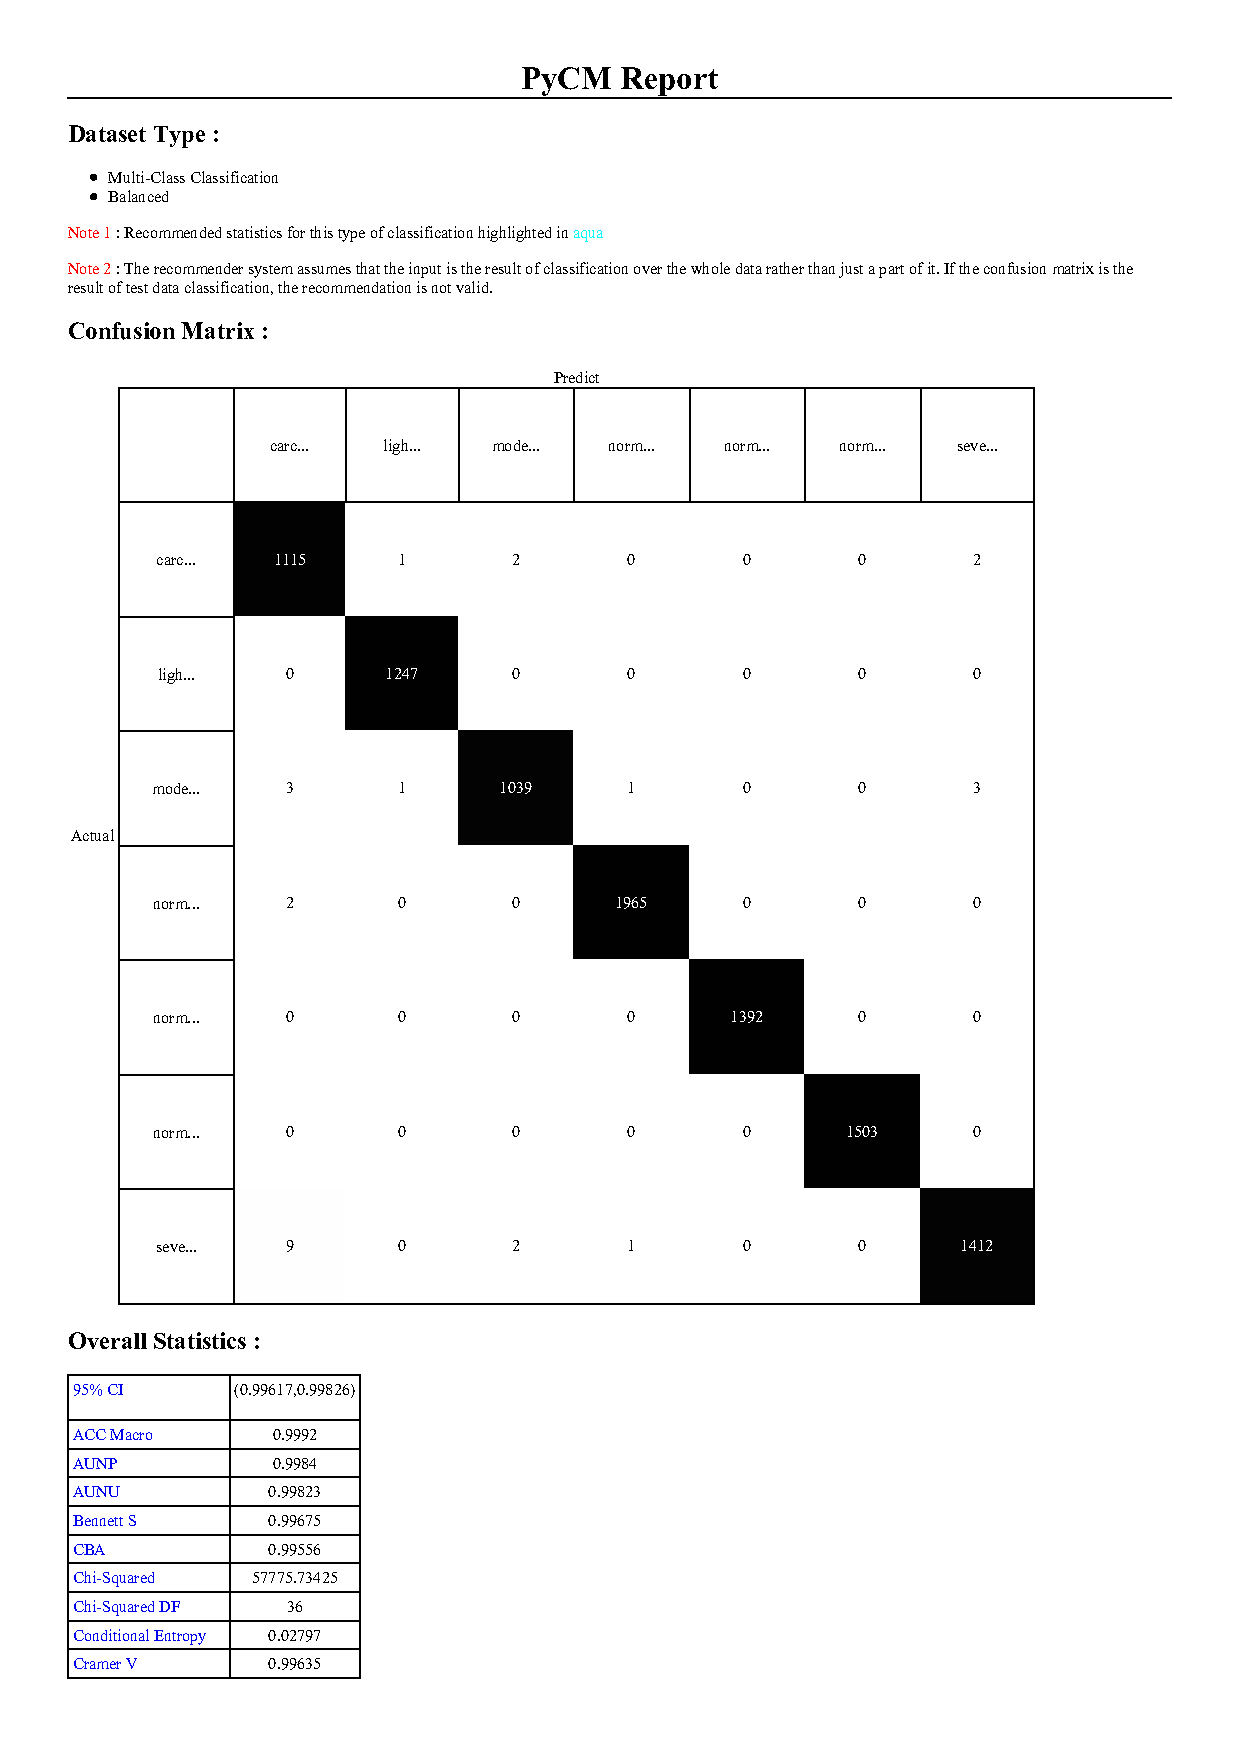
\includepdf[pages=-]{capitulos/capitulo_final/reporte_html.pdf}

